\chapter{Communication}

Different communications are detailed in this chapter, such as particle and 
frontier communications.

\section{Particle communication}

When the particles are moved, due to the interaction with the electric field and 
the magnetic field, their position can exceed the boundaries of the chunk where 
they reside. After updating the position of each particle, the ones that exceed 
the chunk must be translated to the correct one. The process of particle 
communication is done in two stages: first the particles are moved in the X 
dimension, then in the Y. Several steps are required in each stage.

\subsection{Exchange in X}
%TODO Place figure to describe the movement
All chunks in the X dimension reside in one MPI process, so the exchange of 
particles can be done by shared memory. Care must be taken to avoid concurrent 
writes in the same chunk by different tasks. The proposed solution avoids the 
problem by using temporal queues in each chunk. The process can be described in 
the following steps:
%
\begin{enumerate}
\item \texttt{collect\_particles\_x}: Out of bound particles in the X direction 
are extracted from the chunk and placed in the correct target chunk queue for 
local exchange.
\item \texttt{exchange\_particles\_x}: Each chunk looks for particles in the 
neighbour chunks target queues and moves them to itself.
\end{enumerate}
%
Usually only two target queues are required for each chunk, as the particles can 
only move one chunk per iteration. However, in the initial iteration after the 
initialization of the particle positions, they can move to any other chunk, and 
the process is subsequently more computationally expensive. We will only focus 
in the general case involving only the two neighbours, as the initialization 
iteration can be disregarded when comparing the time against the whole 
simulation.

% TODO:Should we split this details in another section/chapter involving only
% tasks and TAMPI?
Each step can be implemented using tasks with dependencies, in order to exploit 
local parallelism. One task collects the particles out of the chunk in the 
corresponding queues, so it needs to access only the current chunk.
%
\begin{lstlisting}
for(i = 0; i < plasma->nchunks; i++)
{
	chunk = &plasma->chunks[i];
	/* Place each particle outside a chunk in the X dimension, in
	 * the lout list */
	#pragma oss task inout(*chunk) label(collect_particles_x)
	for(is = 0; is < sim->nspecies; is++)
	{
		collect_particles_x(sim, chunk, is, global_exchange);
	}
}
\end{lstlisting}
%
The exchange process can now run in parallel, but the task can only run if the 
collecting process has finished in the neighbour chunks, as otherwise the queues 
are still being written. The dependencies can be placed in all involved chunks.
%
\begin{lstlisting}
for (i = 0; i < plasma->nchunks; i++)
{
	chunk = &plasma->chunks[i];
	...

	#pragma oss task inout(*chunk) \
@          inout(*prev_chunk) inout(*next_chunk) \
@          label(exchange_particles_x)
	{
		/* Only the two neighbours are needed */
		concat_particles(chunk, prev_chunk);
		concat_particles(chunk, next_chunk);
	}
}
\end{lstlisting}
%
Notice that in the first iteration the exchange step must wait for all the 
collecting tasks to finish, as the particles can be moved to any chunk, and thus 
we expect to see a slower iteration than the rest of the simulation. In the 
following steps, only the neighbours at $i-1$, $i$ and $i+1$ are required to 
finish the exchange process.

\begin{figure}[h]
	\centering
	\subfloat[Chain of dependencies observed]{
		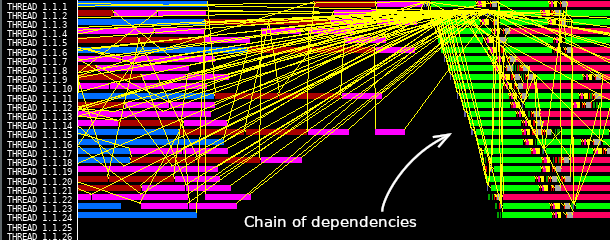
\includegraphics[width=0.7\textwidth]{chain}
		\label{fig:chain}
	}
	\\
	\subfloat[The chain has been corrected]{
		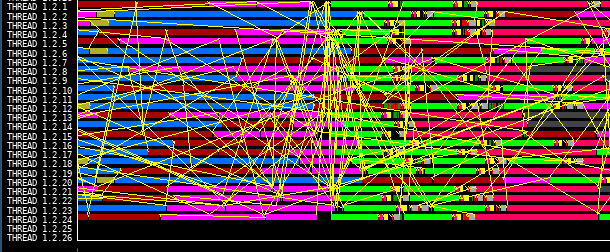
\includegraphics[width=0.7\textwidth]{no-chain}
		\label{fig:no-chain}
	}
	\caption{Comparison of two \texttt{paraver} traces using coloring tasks for 
	communication.}
\end{figure}
%
However, there is a problem with the previous loop: as we create the 
dependencies with the next chunk before the next task is created, we are 
building a chain. Using \texttt{paraver} we can clearly see the chain in the 
trace graph, shown in the figure~\ref{fig:chain}, where no task can run in 
parallel until the previous one finishes.  One solution to alleviate this 
problem is the use of colors, where the loops creates all tasks of the same 
color first, then the ones with the next color and so on.  With three colors we 
ensure that the two tasks of the same color can run in parallel without 
concurrent access to the same chunk.
%
\begin{lstlisting}
max_color = 3;

for(color = 0; color < max_color; color++)
{
	/* Use coloring to prevent a chain of dependencies */
	for(i = color; i < plasma->nchunks; i+=max_color)
	{
		chunk = &plasma->chunks[i];
		...

		#pragma oss task inout(*chunk) \
	@              inout(*prev_chunk) inout(*next_chunk) \
	@              label(collect_local_particles)
		{
			/* Only the two neighbours are needed */
			concat_particles(chunk, prev_chunk);
			concat_particles(chunk, next_chunk);
		}
	}
}
\end{lstlisting}
%
In the figure~\ref{fig:no-chain} we can now observe how the chain has 
disappeared, and the holes are now fully covered by tasks running in parallel.

Once all exchange tasks are completed, all particles are now placed in the 
correct chunk in the X dimension, and only the Y movement is left.

\subsection{Exchange in Y}
%TODO Place figure to describe the movement
Once the particles are placed in the correct chunk in the X dimension, the 
displacement to the correct chunk in the Y dimension involves sending the 
particles to another MPI process. The steps can be resumed as
%
\begin{enumerate}
\item \texttt{collect\_particles\_y}: Place each particle out of the chunk 
bounds in a queue (one for each target destination).
\item \texttt{pack\_particles\_y}: Pack the particles to be sent to the 
neighbour chunk in a message.
\item \texttt{send\_particles\_y}: Send the packed particles to each neighbour.
\item \texttt{recv\_particles\_y}: Receive the message with the packed 
particles.
\item \texttt{unpack\_particles\_y}: Unpack the particle message and place the 
particles in the chunk.
\end{enumerate}
%
\begin{figure}
\centering
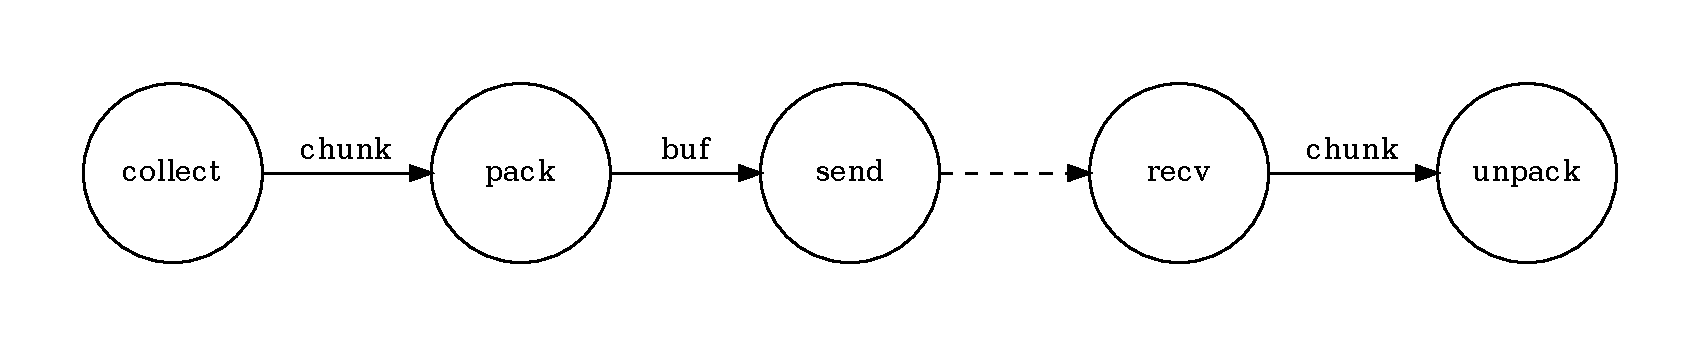
\includegraphics[width=\textwidth]{comm-particles.pdf}
\caption{Graph of task and dependencies of particle communication in 
Y}
\label{fig:comm_y}
\end{figure}
%
Similarly as for the horizontal direction, the particles exceeding the limits of 
each chunk in the Y dimension are placed in a queue.  Once the particles are 
identified within a chunk, they are packed in a message in a contiguous memory 
region. This buffer is then sent using \texttt{MPI\_Send} to the neighbour 
process.

The reception process works in the opposite order: each chunk receives the 
communication of the neighbour chunks in the vertical direction. Once a message 
is received is unpacked and the particles are added to the chunk. In the 
diagram~\ref{fig:comm_y} the dependencies of each step are shown in a graph.

Notice that all the MPI communication is independent of the neighbour chunks in 
the horizontal direction, and can be fully parallelized. Some constraints must 
be added to coordinate the vertical communications to guarantee that no 
simultaneous writes occur in the same chunk.

\begin{lstlisting}
for(i = 0; i < plasma->nchunks; i++)
{
	chunk = &plasma->chunks[i];

	/* Collect particles in a queue that need to change chunk */
	#pragma oss task inout(*chunk) label(collect_particles_y)
	for(is = 0; is < sim->nspecies; is++)
	{
		collect_particles_y(sim, chunk, is, global_exchange);
	}

	/* Prepare the packet to be sent to the neighbour */
	#pragma oss task inout(*chunk) label(pack_particles_y)
	pack_particles_y(sim, chunk, i, global_exchange);

	/* Finally send the packet */
	#pragma oss task in(*chunk) label(send_particles_y_y)
	send_particles_y(sim, chunk, i, global_exchange);

	/* We cannot create here a task as we don't know the dependencies
	 * when using MPI */
	recv_particles_y(sim, chunk, global_exchange);
}
\end{lstlisting}
